La componente relativa all'unita viene sviluppata utilizzando il run-time \glock{Node.js} ed i \glock{WebSocket} per la comunicazione con le componenti del server e dei sensori.
La scelta architetturale per questa componente é ricaduta sulla \textit{Hexagonal Architecture}. \\
I motivi riconducibili alla suddetta scelta sono da riscontrarsi nel tipo di sviluppo che si é deciso di seguire: in un primo momento si sono definite le logiche interne della componente, che risultano essere molto semplici e non richiedono l'utilizzo di librerie esterne. Successivamente si é passati a definire tutte le possibili informazioni che la componente può voler scambiare con le altre e, sulla base di questa modellazione si sono definite le interfacce \textit{UseCase} e le loro implementazioni \textit{Service}. In particolare, questo risultava coerente con il modello di sviluppo che sottende il pattern architetturale: definire la business logic non curandosi di come le informazioni verranno scambiate tra le componenti, e poi utilizzare la stessa per gestire i flussi di informazioni modellandoli a partire dagli \textit{UseCase} proposti (nel nostro caso, gli \textit{UseCase} collimano con i messaggi che l'unità invia e riceve).
É inoltre prevista, similmente a quanto accade per la parte relativa alla UI, una gerarchia di interfacce e classi che si occupano di modellare tutti i possibili messaggi che l'unità può voler scambiare con le altre componenti, in modo da controllare in maniera più pulita il messaggio di informazioni tra i layer interni. \\
Per simulare la rilevazione di ostacoli da parte delle unità si utilizzerà il componente Sensors. Essendo di dimensioni minime, non è stato seguito un particolare design pattern.

\begin{figure}[H]
	\centering
	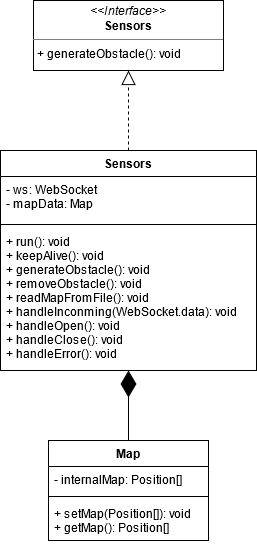
\includegraphics[width=4cm]{img/unit_sensori.png}
	\caption{Unità - Sensori}
\end{figure}

Di seguito si illustrano i diagrammi delle classi dell'architettura dell'unità, e dei messaggi usati per interfacciarsi con il server.

\begin{landscape}
	\begin{figure}[h!]
		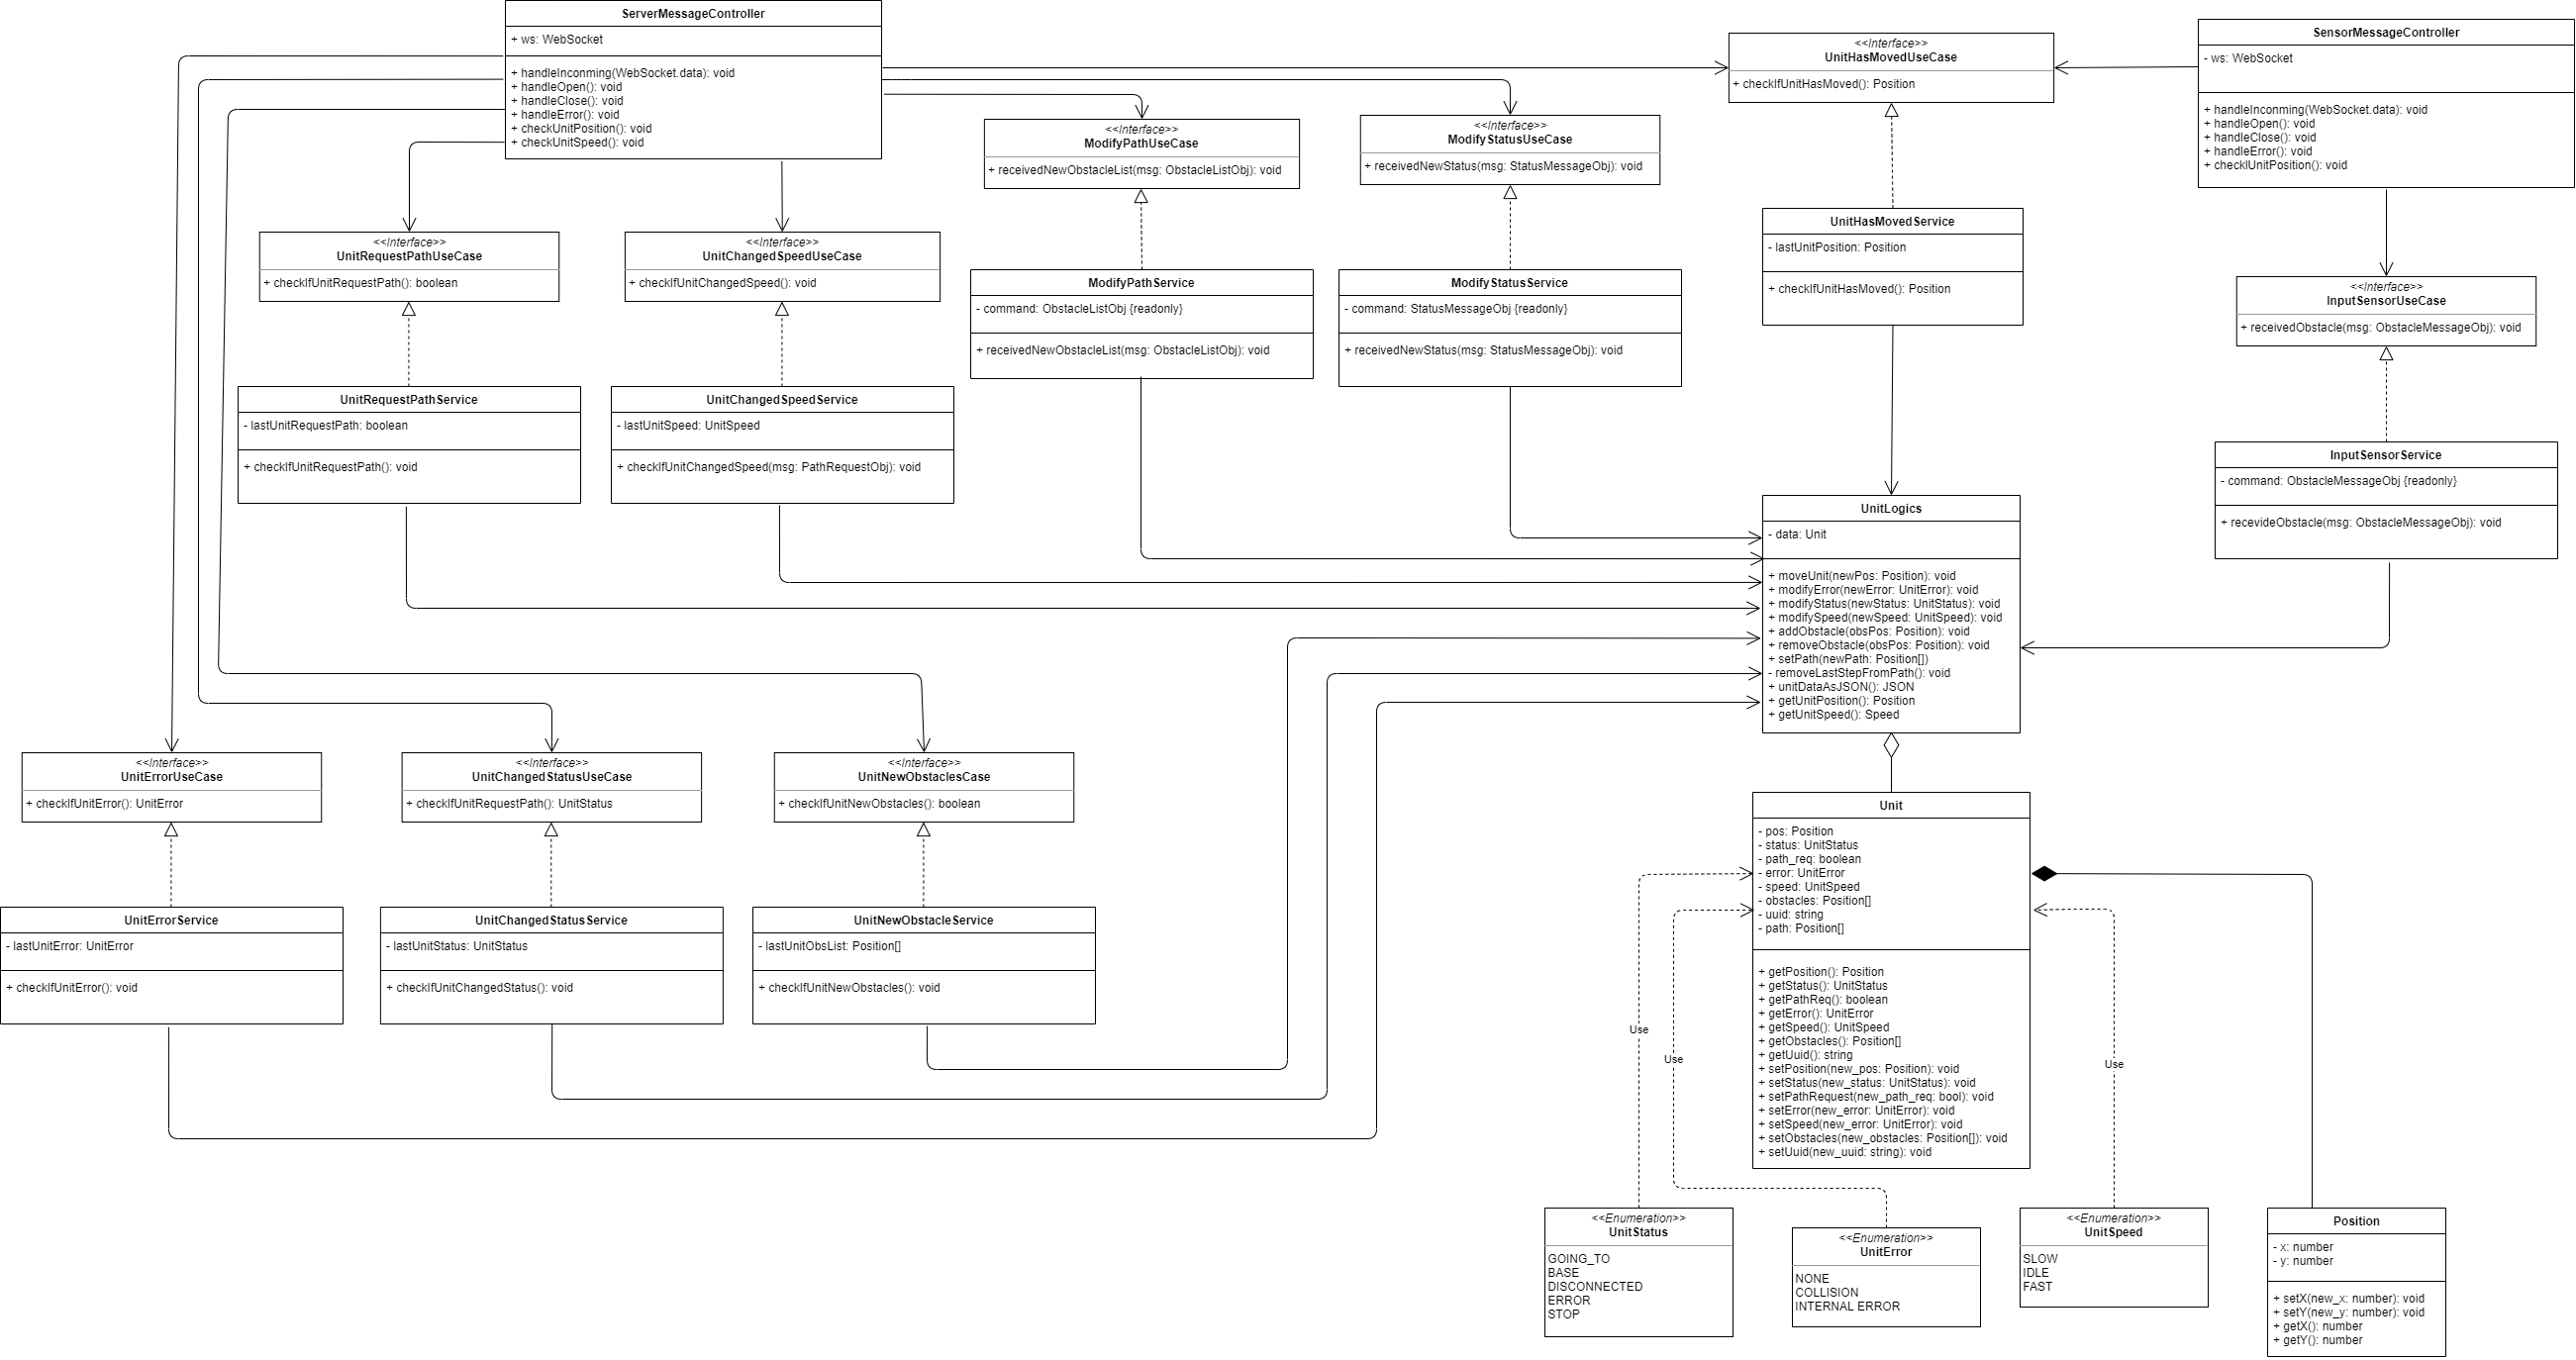
\includegraphics[width=24cm]{img/unit_architettura.png}
		\caption{Unità - Diagramma delle classi}
	\end{figure}
\end{landscape}

\begin{figure}[H]
	\centering
	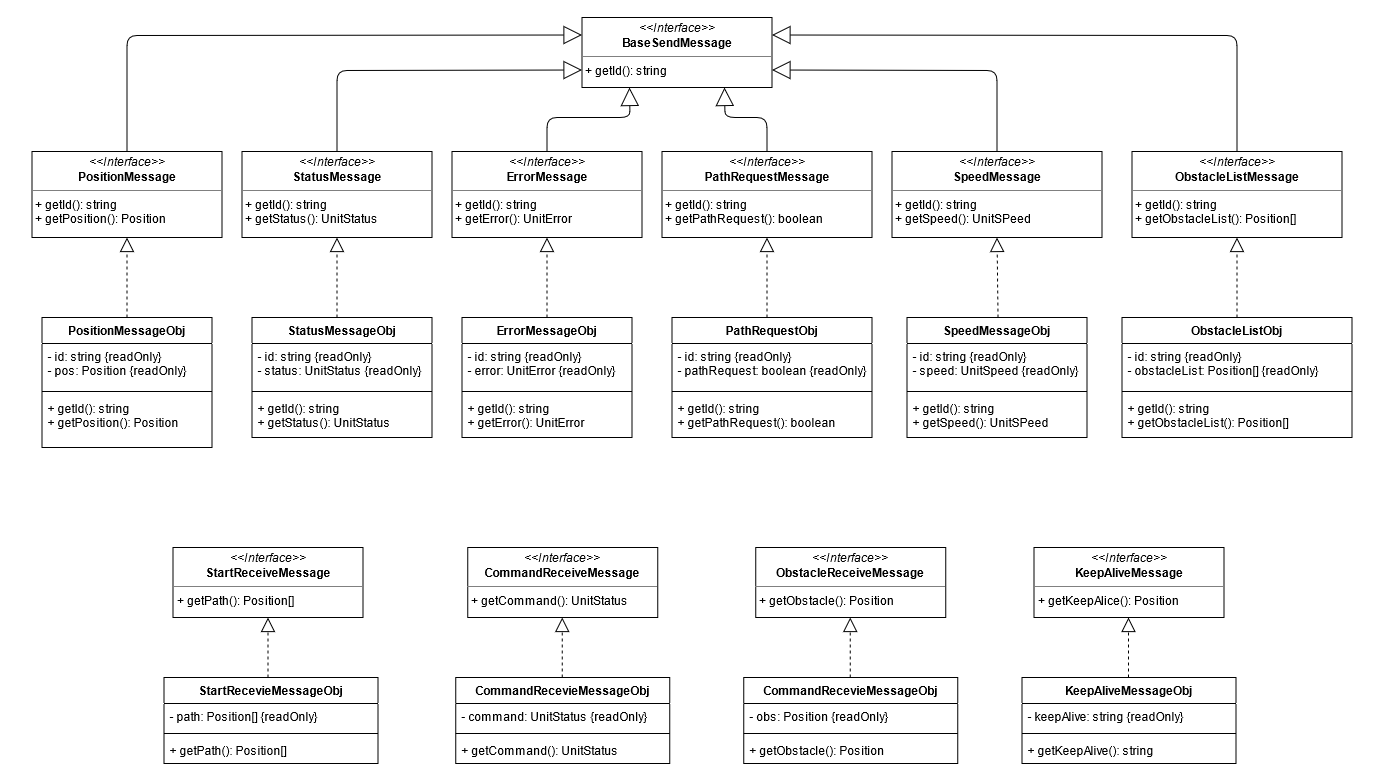
\includegraphics[width=18cm]{img/unit_messaggi.png}
	\caption{Unità - Messaggi}
\end{figure}